\documentclass[a4paper,12pt]{report}
\usepackage[utf8]{inputenc}
\usepackage{times}
\usepackage{graphicx}
\usepackage{url}
\usepackage{amsmath}
\usepackage{array}
\usepackage{mathtools}
\usepackage{ifthen}
\usepackage{mathrsfs}
\usepackage{setspace}

\oddsidemargin 0.6in		% Left margin is 1in + this value
\textwidth 5.in		% Right margin is not set explicitly
\topmargin 0.25in			% Top margin is 1in + this value
\textheight 8.in			% Bottom margin is not set explicitly
%\setlength{\columnsep}{2cm}



\iffalse
These words need to be added to the dictionary:
Ginzburg, soliton, Runge, Kutta, CGLE, Fourier, Landau nonlinearity
discretise nonlinear, NLSE, solitons, Coursera
Benard superfluidity saturable nonlinearities
Schrodinger Hohenberg Hausdorff Mathematica Nyquist
SVM overfitting sech Akhmediev Ankiewicz
Schodinger pseudospectral
I will use nonlinear (not non linear or non-linear)
\fi


\iffalse
Before I submit, make sure I check that the following have updated themselves properly.
Spell Check
Contents Page
Image reference numbers
Table reference numbers
Citation numbers
make sure bibliography is on contents page (once)
\fi






\begin{document}
\begin{titlepage}
\centering
{\ \\ }
\vspace{3cm}
{\bf  \fontsize{1.35cm}{2.5cm}\selectfont \vspace{0.5cm} Using Machine\vspace{0.5cm} Learning to \vspace{0.5cm}Predict Properties\vspace{0.5cm} of Soliton Solutions of\vspace{0.5cm} the Complex \vspace{0.5cm}Ginzburg Landau Equation\vspace{0.5cm}}\\
%\vspace{2cm} \\
{\Huge By Max Proft}\\
{\Huge u5190335}
\end{titlepage}










\newcommand{\unnum}[2]{
\ifthenelse{\equal{#1}{chapter}}{\chapter*{#2}}{
\ifthenelse{\equal{#1}{section}}{\section*{#2}}{
\ifthenelse{\equal{#1}{subsection}}{\subsection*{#2}}
{\chapter*{ERROR: #2}}}}
\addcontentsline{toc}{#1}{#2} 
}%This is the exception if no case matches!!!
\tableofcontents{}
\iffalse
The order is:
Chapter
Section
Subsection
Subsubsection (not shown in contents)
\fi



\onehalfspacing


\unnum{chapter}{Abstract}
A program was written to produce soliton solutions of the complex Ginzburg Landau equation. Various ways to solve this program were explored, ultimately resulting in it being numerically solved with a split step Fourier and Runge Kutta method. A range of previously published solitons were successfully replicated. 
\\\\
Various machine learning techniques were learnt and polynomial regression was then used to predict properties of solitons. Various properties were tried, however the only property that could be reliably predicted was the height of a soliton. 92\% of the stationary solitons were able to have their height predicted within 2\% of the true value, and 95\% of the pulsating solitons were able to have their height predicted within 5\%  Various reasons were explored as to why this may other properties could not be predicted, and suggestions for future projects involving machine learning to predict soliton properties were given. 

\unnum{chapter}{Acknowledgements}
I would like to thank Nail Akhmediev and Adrian Ankiewicz for pointing me in the right direction when I got stuck. I would also like to thank my friends who I was able to discuss machine learning with, as well as everyone else for putting up with me over the past 4 years. 


\chapter{Introduction to the Complex Ginzburg Landau Equation}
The complex Ginzburg Landau equation (CGLE) is a differential equation that is typically written in the following form: 
$$i\psi_t +\frac{D}{2}\nabla^2\psi+|\psi|^2\psi +\nu |\psi|^4\psi = i\delta \psi+i\epsilon|\psi|^2\psi +i\beta\nabla^2\psi+i\mu|\psi|^4\psi$$
This equation describes the evolution of a number of systems, from quantum systems like superconductivity and superfluidity near phase transitions \cite{annett}, as well as classical systems like Rayleigh Benard convection\cite{wocgle} and fibre optic propagation in mode locked lasers\cite{2001}. Different systems give the CGLE for different numbers of spatial dimensions and in this thesis we consider the case where $\nabla^2\psi=\frac{\partial \psi}{\partial x^2}$ which is the case for mode locked lasers. 
\\\\
The CGLE is an amplitude equation, which means that the quantity we are modelling (e.g. intensity) is given by $|\psi(x,t)|^2$ and energy given by $\int|\psi(x,t)|^2 dx$, albeit with scaling. 
$D$ describes the group velocity dispersion, and is typically taken to be $1$ for normal dispersion or $-1$ for anomalous dispersion. Dispersion is considered normal if when the optical frequency is increased, the group velocity is seen to decrease. The dispersion is anomalous when the relationship between the optical frequency and group velocity is reversed. It should be noted though that $D$ is not always taken to be $\pm1$\cite{spiny,spike}. 
Parabolic gain and spectral filtering is represented by $\beta>0$. 
$\delta$ is the linear gain-loss. 
$\epsilon$ represents the nonlinear gain which can arise for a variety of reasons such as saturable absorption, which describes how the rate of absorption decreases as the  intensity increases.
$\mu$ and $\nu$ describe higher order nonlinearities such as the saturation of the nonlinear gain and a nonlinear refractive index respectively. \cite{2001}
\\\\
The CGLE gives rise to localised formations called solitons. Solitons occur when the diffraction or dispersion is cancelled out by the nonlinearity of the system. Additionally, the CGLE describes dissipative phenomena, and so energy is not conserved. This means that for solitons to be stable the loss and gain must cancel out on average. \cite{dissys}
\\\\
The CGLE is often written without the quintic terms ($|\psi|^4\psi$) however it has been shown that these higher order terms are often needed for solitons to be stable in the 1D case. \cite{5th}



\section{Origins of the CGLE}
The CGLE describes a wide range of phenomena. Upon setting various components to zero, we get the nonlinear Schrodinger equation as well as fluid dynamics equations such as the diffusion equation. This lead Aronson and Kramer\cite{wocgle} to consider the CGLE as an extension to the nonlinear Schrodinger equation that allows for dissipation and higher order nonlinearities.  
\\
\\
A heuristic way of deriving the CGLE is by trying to find a general differential equation which is invariant under multiplication by a phase shift $e^{i\phi}$.\cite{hecke} This leaves few choices for the differential equation. 
First off, any derivative will satisfy this condition. If we assume that the $\psi$ is sufficiently smooth or that the dispersion and parabolic gain is dominant, we can ignore derivatives with order greater than 2. As shown in the next paragraph, we are able to rescale our system to remove first order derivatives. Additional functions can be approximated with a Taylor expansion in terms of $\psi$ and $\psi^*$, with these elements are given by $\{\psi,\psi^*, \psi^*\psi, \psi\psi\psi^*,\psi\psi^*\psi^*, ...\}$. Of these terms, the only ones that are able to satisfy invariance under a phase shift, $\psi\rightarrow \psi e^{i\phi}$, are the terms that take the form $|\psi|^{2n}\psi$ for some positive integer n. 
\\
\\
Aranson and Kramer\cite{wocgle} explicitly derive the CGLE from a general set of hydrodynamic equations. The hydrodynamic equations are able to model a range of fluid phenomena, such as Rayleigh-Benard convection cells that are formed by heating a fluid from underneath. This hydrodynamic equation is given as:
$$\tau (\partial_{\tilde t}\tilde A-\tilde v_g\cdot \tilde\nabla \tilde A)=\epsilon(1+ia)\tilde A+\xi^2(1+ib)\tilde\nabla^2 \tilde A-g(1+ic)|\tilde A|^2 \tilde A$$ 
This equation can be rescaled with the following transformations to get the CGLE: 
$$\tilde A=(\epsilon/g)^{1/2} A \ exp[-i (\epsilon a/\tau)\tilde t], \ \ \tilde t = (\tau/\epsilon)t, \ \ \vec {\tilde x} = (\xi/\epsilon^{1/2})\vec x+\vec v_g \tilde t$$
When substituting this in, we get the CGLE up to the cubic terms:
$$\partial_t A=A+(1+ib)\nabla^2A-(1+ic)|A|^2A$$
If the hydrodynamic equation was generalised to have higher order nonlinearities, using the same transformations the quintic term needs to be multiplied by $ \frac{\epsilon}{g^2} $ to get the appropriate scaling.
\\
\\
%As a final example, the CGLE is able to describe superconductivity near a superconducting transition. The intensity is given by $F=F_n +\alpha |\psi|^2+\frac{\beta}{2}|\psi|^4 +\frac{1}{2m}|(-i\hbar\nabla -2eA)\psi|^2+\frac{|B|^2}{2\mu_0}$, where $B$ and $A$ are the magnetic field and vector potential. The evolution equation is found with the following equation, and if there is no magnetic field the equation simplifies to the CGLE. 
%$$\partial_t \psi = -\frac{\delta F}{\delta \psi^*} $$









\chapter{Mathematical Theory Behind Solving the CGLE}
\section{A Brief Look at Different Methods to Solve the CGLE}
Although some specific exact solutions have been found which solve the CGLE for specific parameter values\cite{exact}, in general it cannot be solved exactly and so numerical methods must be used instead. 
\\
\\
A finite difference method was used initially before a better method was chosen. The key idea behind a finite difference method is to approximate spatial derivatives with $\frac{\partial \psi}{ \partial x}\approx \frac{\Delta \psi}{\Delta x}$. Given that $|\Delta \psi|\ll |\psi|$, the spatial derivatives will end up losing several digits of precision. Additionally, if there are sharp peaks and slowly varying features, then $\Delta x$ must be very small to ensure that the features are represented accurately, which leads the precision of $\Delta \psi$ to become even worse for the slow changing features. However there are a number of other ways for the CGLE to be solved. 
\\
\\
Taha and Ablowitz \cite{taha} compared various methods for solving the nonlinear Schrodinger equation. Given that the CGLE can be seen as an extension of the nonlinear Schrodinger equation, we would expect to draw a comparable conclusion when solving the CGLE instead. 
\\
\\
One method given was a pseudospectral method. This method involves replacing $\nabla^2\psi$ with $F^{-1}(-(2\pi f)^2F(\psi))$, where $F$ and $F^{-1}$ refer to the Fourier transform. Then the differential equation, $\frac{\partial \psi}{\partial t}=f(\psi)$, is evolved forwards with the step equation $\psi\rightarrow\psi+f(\psi)\Delta t$, for some small time step $\Delta t$.
\\\\
Another method given was the Ablowitz-Lodik global scheme. They conjectured that it would be a faster method for high amplitude solitons, however many solitons do not contain large amplitudes so there is no benefit in using this method. 
\\
\\
Overall a split step Fourier method was found to be the fastest algorithm. For the CGLE this method needs to be adjusted as the quintic terms prevent it from being possible to solve in the same way. This leads to the Runge Kutta method being used as part of this split step method, which has also been done previously. \cite{2001,spiny,spike,extreme,bch}



\section{Split Step Fourier and Runge-Kutta Method}
In this section, the CGLE will be written in the following way in order to aid clarity of reading. The equation can be split into linear and nonlinear parts:
$$\frac{\partial\psi}{\partial t} = A \frac{\partial^2\psi}{\partial x^2} + B\psi + C |\psi|^2\psi + D|\psi|^4\psi = \hat L \psi + \hat N \psi$$
where the linear component is:
$$\hat L \psi = A \frac{\partial^2\psi}{\partial x^2} + B\psi$$
and the nonlinear component is:
$$\hat N \psi = C |\psi|^2\psi + D|\psi|^4\psi$$
The split step Fourier and Runge Kutta method assumes that the linear and nonlinear terms do not significantly affect each other over short time scales.\cite{taha} This means that we can propagate forwards according to the linear evolution equation, and then propagate forwards according to the nonlinear evolution equation. When the time step is sufficiently small this will be a good approximation for the solution to the original differential equation. For a small time step this can be represented with the following:
$$\psi(t+\Delta t)=e^{\hat N\Delta t+\hat L\Delta t}\psi(t)\approx e^{\hat N\Delta t}e^{\hat L\Delta t}\psi(t)$$ 
This formula is a limit of the Baker Campbell Hausdorff formula under the limit that $\Delta t\rightarrow 0$.
Furthermore, this formula can be adjusted in the following way to make the solution more stable. \cite{bch}
$$\psi(t+\Delta t)=e^{\hat N\Delta t/2}e^{\hat L\Delta t}e^{\hat N\Delta t/2}\psi(t)$$ 





\subsection{Linear Evolution (Fourier) \cite{taha}}
In this section the following equation will be solved:
$$\frac{\partial\psi}{\partial t}=A\frac{\partial^2\psi}{\partial x^2}+B\psi$$
The Fourier transform will be defined as: 
$$\hat \psi(f)=\int\limits_{-\infty}^\infty \psi(x)e^{-i2\pi x f} dx$$
By taking the Fourier transform of both sides, the differential equation becomes:\\
$$\frac{\partial \hat \psi}{\partial t}= (-2\pi i f)^2 A \ \hat \psi (f)+B\ \hat \psi(f)= (B-A \ 4 \pi^2 f^2) \hat \psi(f)$$
$$\implies \hat \psi_t(f) = e^{(B-A \ 4\pi^2 f^2)t}\hat \psi_0(f)$$
Where $\hat \psi_t(f)$ is the Fourier transform at time $t$.
By taking the inverse Fourier transform of both sides of this equation, the differential equation can be solved. 
The Fourier transform can be done numerically approximated by using a discrete Fourier transform.






\subsection{The Relationship Between the Fourier Transform and Discrete Fourier Transform}
Below the relationship between a Fourier transform and a discrete Fourier transform is derived. While the explanation given can be adjusted for periodic boundary conditions, it is easier to show the relationship if it is assumed that the function is zero outside of some domain. With this assumption, the Fourier transform can be written as:
$$\tilde \psi(f) = \int_{-\infty}^\infty \psi(x) e^{-i2\pi xf} dx \approx \int_0^L\psi(x)e^{-i2\pi x f}dx$$
Let $\Delta x=L/N$ for some integer $N$. The Fourier transform can then be approximated by:
$$\approx \sum\limits_{n=0}^{N-1}\psi(n \Delta x) e^{-i 2\pi n \Delta x f}\Delta x$$
Let $\Delta f = (f_1-f_0)/N$, for some values of $f_1$ and $f_2$. With the same reasoning as before, the inverse Fourier transform can be approximated as the following:
$$\psi(x) = \int_{-\infty}^\infty \tilde\psi(f)e^{i 2\pi x f} df \approx \int_{f_0}^{f_1}\tilde\psi(f)e^{i 2\pi x f}df $$
$$\approx \sum\limits_{m=0}^{N-1}\tilde\psi(f_0+m\Delta f)e^{i 2\pi n\Delta x f_0} e^{i 2\pi x m\Delta f}\Delta f$$
Let $\psi(n\Delta x) = \psi_n$ and $\tilde\psi(f_0+m\Delta f) = \tilde \psi_m$
$$\tilde \psi_m\approx \Delta x \sum\limits_{n=0}^{N-1}\psi_n e^{-i 2\pi n \Delta x f_0}e^{-i 2\pi n m \Delta x \Delta f}$$
$$\psi_n  \approx \Delta f e^{i 2\pi n\Delta x f_0}\sum\limits_{m=0}^{N-1}\tilde\psi_m e^{i 2\pi n m \Delta x \Delta f}$$
The frequency difference should correspond to difference between adjacent elements, giving $f_1-f_0=1/\Delta x$. This means that $\Delta f = 1/(N\Delta x)$. The Nyquist sampling theorem says that for a set of equally spaced data sampled from a signal, the highest frequency that can be reproduced is half of the sampling frequency, and so $f_0=\frac{-1}{2\Delta x}$. This allows the approximation of the Fourier transform to be further simplified:
$$\tilde \psi_m\approx \Delta x \sum\limits_{n=0}^{N-1}\psi_n e^{i \pi n }e^{-i 2\pi n m/N}=\Delta x \sum\limits_{n=0}^{N-1}\psi_n (-1)^n e^{-i 2\pi n m/N}$$
$$\psi_n  \approx \frac{e^{-i \pi n}}{N\Delta x}\sum\limits_{m=0}^{N-1}\tilde\psi_m e^{i 2\pi n m/N}=\frac{(-1)^n }{N\Delta x}\sum\limits_{m=0}^{N-1}\tilde\psi_m e^{i 2\pi n m/N}$$
The discrete Fourier transform and its inverse is defined in the following way:
$$\tilde A_m =  \sum\limits_{n=0}^{N-1} A_n e^{-i 2\pi n m/N}$$
$$A_n  = \frac{1}{N}\sum\limits_{m=0}^{N-1}\tilde A_m e^{i 2\pi n m/N}$$
Hence the (inverse) Fourier transform can be computed using a discrete (inverse) Fourier transform providing that the data is multiplied element-wise by the appropriate constant. 
\\
\\
The main limitation of this method occurs if the sampling rate is too low. When this happens, aliasing can occur which will causes the frequencies found with the Fourier transform to have the wrong amplitudes, as demonstrated in figure \ref{aliasing}.
\begin{figure}[h]
\centering
\includegraphics[width=3.6in]{aliasing}
\caption{A small sampling rate can result in the aliasing of the function. This leads to the amplitudes of the frequencies being wrong, and hence the function will not evolve correctly in time.}
\label{aliasing} 
\end{figure}





\subsection{Nonlinear Evolution (Runge-Kutta) \cite{boyce}}
In this section, the following equation will be solved:
$$\frac{\partial\psi}{\partial t}=C|\psi|^2\psi + D|\psi|^4\psi$$
The Runge Kutta method is used to numerically solve any first order differential equation which takes on the form $\frac{d\psi}{dt}=f(t,\psi)$. It is similar to the Euler method, which solves equations with the following step equations for some small time step $\Delta t$:
$$\psi\rightarrow \psi + f(t,\psi)\Delta t $$
$$t\rightarrow t+\Delta t$$
The Runge Kutta method has better convergence than the Euler method, and has an error of $O(\Delta t^5)$, compared with $O(\Delta t^2)$. 
\\\\
The first step of the Runge Kutta method is to define $f(t,\psi)=C|\psi|^2 \psi  +D|\psi|^4 \psi$. Next, the initial conditions, step size and the total number of steps to be taken need to be chosen.
For each iteration, we define the following:
$$K_1 =f(t,\psi)$$
$$K_2 =f(t+\Delta t/2,\psi+K_1 \Delta t/2)$$
$$K_3 =f(t+\Delta t/2,\psi+K_2 \Delta t/2)$$
$$K_4 =f(t+\Delta t,\psi+K_3\Delta t)$$
Finally, $\psi$ and $t$ are evolved forwards in time by updating the system in the following way:
$$t\rightarrow t+\Delta t$$
$$\psi\rightarrow \psi+(K_1+2K_2+2K_3+K_4) \ \ \Delta t/6$$


\begin{figure}[h]
\hspace*{-1.cm}
%\centering
\includegraphics[width=5.8in]{goodbadres}
\caption{Above the CGLE has been solved with the same initial conditions and with parameters $\epsilon=1.0,\ \delta=-0.1,\ D=1, \ \beta=0.125, \ \mu=-0.1,\ \nu=-0.6$\cite{2001}. The left and right images has $t$ steps of 0.02 and 0.01 respectively, resulting in significantly different solutions.}
\label{goodbadres} 
\end{figure}
\section{Testing the Code}
The linear and nonlinear step equations were individually compared with a numerical result from Mathematica to ensure that this implementation was done correctly. Next the program was compared to an exact solution of the nonlinear Schrodinger equation to ensure that the split step component was implemented correctly. 
Finally, there are a number of papers which give interesting solutions to the CGLE, and these were reproduced as elaborated in a later chapter. This was able to give confidence that this algorithm was correctly implemented. 
Finally, it is important to note that if an interesting soliton is found, it may end up simply being an artefact of a large step size, as in figure \ref{goodbadres}. If the step size and spatial resolution are improved and the resultant soliton does not significantly change, then this can be claimed as a solution to the CGLE.



% While many explicit solutions for the nonlinear Schrodinger equation have been found, with additional nonlinearity means that finding explicit solutions to the CGLE is often not possible.
%\\\\
%(Jia-Min Zhu and Zheng-Yi Ma (2007),Pierre Hillion (2012), Mihalache and Panoiu (1992), Yan-Ze Peng and Krishnan (2007) =  Schrodinger equation)





\chapter{Machine Learning Theory}
Since the CGLE has 6 parameters that can be varied, if 100 data points were taken over a given range for each parameter there would be $10^{12}$ different solutions that would need to be calculated. Given that each solution takes on the order of a minute each, this cannot be done. In the past, people have only varied one or two parameters at a time and have eneded to draw conclusions from this small slice of the sample space.\cite{2001, spiny, spike, extreme} Instead of explicitly trying to calculate a vast number of solitons for a wide range of parameters it may be possible to use machine learning to predict information about these solitons.




\section{Different Types of Machine Learning}
As part of my thesis, I did the online machine learning course by Stanford University. \cite{mooc} This course covered a number of techniques such as linear regression, neural networks, support vector machines, principle component analysis, k-means clustering, anomaly detection and recommender systems. Below is a summary of the methods covered.
\\\\
Linear Regression: Good for predicting a specific value. Given the input parameters, we want to predict a specific value for the output. Polynomial regression is linear regression with polynomial features. This is described in more detail below.
\\\\
Neural Networks: Good for classifying a binary option for complex systems. I.e. does this property hold, yes or no?
\\\\
Support Vector Machine (SVM): Good for classifying a binary option, providing that the boundary is not too unusual. See figure \ref{svmneural} to get an idea as to when a SVM may be a better option than a neural network.
\begin{figure}[h]
\centering
\includegraphics[width=4.6in]{svmneural} 
\caption{Left, an SVM aims to find a boundary to classify the data with. Right, more complicated boundaries can be better modelled with a neural network.}
\label{svmneural} 
\end{figure} 
\\\\
Principle Component Analysis: Suppose there is a 2D plane embedded in 3 dimensions. Principle component analysis provides a method to reduce the dimensionality to two dimensions, and can be generalised to higher dimensions.
\\\\
K-Means Clustering: This technique is used to collect data into groups when you don't know what the groups are, as in figure \ref{kmeans}.
\begin{figure}[h]
\centering
\includegraphics[width=2.6in]{kmeans}
\caption{K-Means Clustering. Initially the number of clusters is guessed. Then the red dots are moved such that they minimise the distance to nearby points. Any new point is part of the cluster whose red dot is closest.}
\label{kmeans} 
\end{figure}
\\\\
Anomaly Detection: The purpose of anomaly detection is to determine whether a set of parameters is unusual. If the distribution of each parameter is not Gaussian, it needs to be transformed to a Gaussian-like distribution. The variables can be either independent of each other or linearly correlated as in figure \ref{anomaly}. This technique is preferred over SVMs and neural networks if there are only a small number of examples of anomalies.
\begin{figure}[h]
\centering
\includegraphics[width=2.6in]{anomaly}
\caption{Anomaly Detection. The data are transformed so that each variable follows a Gaussian-like distribution. In this example, there is a linear correlation between the two variables. The goal of anomaly detection is to be able to return the red dot as an error.}
\label{anomaly} 
\end{figure}
\\\\
Recommender System: Given a customer's previous purchases/etc. what are they likely to want to buy next. This prediction is based on what other, similar people have done.
\\\\
I decided to try and predict properties of solitons such as the energy, width of the soliton, and maximum height. The technique that is best suited for this is polynomial regression. 







\section{Polynomial Regression}
Suppose we have input parameters $\vec x_i$ with the true value of the property to predict being $y_i$. For linear regression, we choose $\vec\theta$ such that our prediction for this value is $\vec\theta \cdot \vec x_i$. We want to vary the vector $\vec \theta$ such that the predictions match as best as possible. This is done by providing a cost function that is lowest when the predictions best match the true value. The least squares cost function is the following, where $(\vec x_i,y_i)$ is the $i^{th}$ example used to train the algorithm.
$$J_\theta = \sum_i \left(\vec\theta\cdot \vec x_i -y_i\right)^2 $$
\begin{figure}[h]
\centering
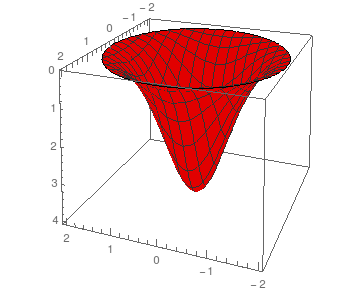
\includegraphics[width=3in]{GradDescent}
\caption{The algorithm finds the minima by continually taking the path with the steepest gradient. For linear regression, the minimum is guaranteed to be unique.}
\label{graddesc}
\end{figure}
\\
Suppose there are two parameters. The cost function may then look something like that in figure \ref{graddesc}.  
The minimum of this graph gives the value of  $\vec\theta$ which gives the best overall prediction. 
Typically the algorithm to find the minimum is done by continually taking the steepest path. Something that might be of concern is whether the algorithm will converge to a local minimum, rather than the global minima. However since the cost function, including the regularised cost function discussed below, is convex, the minimum is unique.
\begin{figure}[h]
\centering
\includegraphics[width=3in]{overfit}
\caption{While the solid blue line fits gives a lower cost, the dashed black line will be more likely to fit new data points well, and so is a better estimate.}
\label{overfit}
\end{figure}
\\\\The number of input features can be increased by adding in an intercept term (i.e. take $x_0=1$ for all training examples) or by adding in polynomial features $\{x_1^2,x_1x_2,x_1x_3, ... \}$. However by adding in these extra features, the algorithm may not accurately represent the true relationship. If there are many polynomial features it becomes much easier to over fit the data as in figure \ref{overfit}. In order to prevent this the cost function can be adjusted by adding in a regularisation term. The cost function then becomes:
$$J_\theta = \frac{1}{2m}\sum_i \left(\vec\theta\cdot \vec x_i -y_i\right)^2 +\frac{\lambda}{2m} |\vec\theta|^2$$
By doing this, if several of the elements of $\vec \theta$ are large, then the cost will increase and this set of parameters will no longer be at the minima. This helps to ensure that only the important features will remain large. For this to not penalise one parameter more than another, the data need to be normalised. This can be done by transforming each feature $x_i^{(j)}$  in the following manner, where the $i$ indicates that it is the $i^{th}$ training example, the $j$ index refers to the $j^{th}$ component of the vector, $\mu^{(j)}$ refers to the mean of the $j^{th}$ component of all the training examples, and $\sigma^{(j)}$ is its standard deviation.
$$x_i^{(j)}\rightarrow \frac{x_i^{(j)}-\mu^{(j)}}{\sigma^{(j)}}$$
This transformation ensures that all of the features are on the same scale, allowing all features to be penalised equally by the cost function. 
\\\\
This algorithm was tested by making data that satisfied $y = 1.5+3.5x_1+3.5x_2x_3$. Unused features were set to random numbers. The algorithm was able to converge to the correct result giving confidence that it has been correctly implemented so it should run appropriately when trained with data from the solitons. 














\chapter{Replication of Previous Results}
Solutions were found by setting the initial state as a Gaussian pulse. This was evolved forwards in time until the transient response was gone. 
Solitons can be categorised into a number of types. First off there are stationary solitons whose profile remains steady in time. Solitons can also be found to pulsate. The simplest type is known as a plain pulsating soliton and is characterised by being periodic, recovering its original shape after a fixed amount of time. An example is given in figure \ref{plain}.\cite{2001}
\begin{figure}[h]
\centering
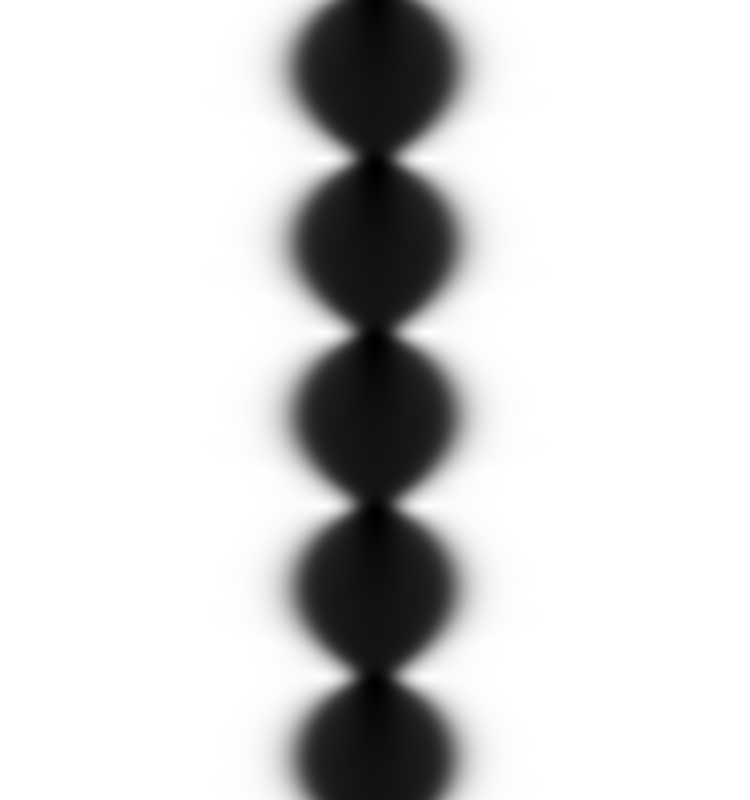
\includegraphics[width=3in]{plain}
\caption{A plain pulsating soliton with parameters $\epsilon=0.66,\ \delta=-0.1,\ D=1, \ \beta=0.08, \ \mu=-0.1,\ \nu=-0.1$. \cite{2001}}
\label{plain} 
\end{figure}
\\\\
Another type of pulsating solitons is known as an exploding or erupting soliton. Ripples and other imperfections can be seen to build up before there is a sharp jump in it's energy profile, as given in figure \ref{exploding}.  Additionally, the time between explosions may be chaotic. \cite{2001}%TODO [40]
\begin{figure}[h]
%\centering
\hspace*{-1.4cm}
\includegraphics[width=6in]{exploding}
\caption{Left: The intensity of an exploding soliton. Right: the energy of the same exploding soliton. The parameters are $\epsilon=1.0,\ \delta=-0.1,\ D=1, \ \beta=0.125, \ \mu=-0.1,\ \nu=-0.6$.\cite{2001}}
\label{exploding} 
\end{figure}
\\
Other pulsating solitons can be periodic and give high intensity spikes. This is seen in figure \ref{highamp} whose energy increases over 10 times because of the spike. \cite{extreme}
\begin{figure}[h]
%\centering
\hspace*{-1.4cm}
\includegraphics[width=6in]{extremepulse}
\caption{A periodic soliton with a high intensity spike. The parameters are $\epsilon=0.95,\ \delta=-0.1,\ D=-1, \ \beta=0.125, \ \mu=-0.0005,\ \nu=0.1$.\cite{extreme}}
\label{highamp} 
\end{figure}
\\\\
High intensity spikes can also have a much narrower width. Some solitons periodically get extremely narrow spikes \cite{spike}, bit it is also possible to get high intensity spikes occurring chaotically, known as a spiny soliton. The intensity profile is given in figure \ref{spiny} along with a zoomed in version of the original soliton.
\begin{figure}[h]
%\centering
\hspace*{-1.4cm}
\includegraphics[width=6in]{spiny}
\caption{A spiny soliton gets high intensity spikes and exhibits a chaotic pattern that resembles noise. The parameters are $\epsilon=0.04,\ \delta=-0.08,\ D=-2.7, \ \beta=0.18, \ \mu=-0.000025,\ \nu=-0.002$.\cite{spiny}}
\label{spiny} 
\end{figure}
\\\\
%By varying parameters, other interesting behaviour can also be seen, such as periodic doubling. Figure \ref{periodicdoubling} 
%TODO
%shows a 1 cycle, 2 cycle, and 4 cycle occur as $\epsilon$ is varied. %figure \ref shows the bifurcation diagram for this process. 
Finally, we can also get pulsating solitons that move, called creeping solitons. An example is given in figure \ref{periodpulse} which in a sinosoial manner, however by varying the initial conditions, it could be made to continually creep right.
%creeps right forever as it oscillates. By varying the initial pulse, but keeping the parameters the same, this pulse can instead be made to creep in sinusoidal way.%TODO creeping, sinusoidal and the two initial pulses. 
%TODO creeping, both sinusoidal and rightwards only
\begin{figure}[h]
\centering
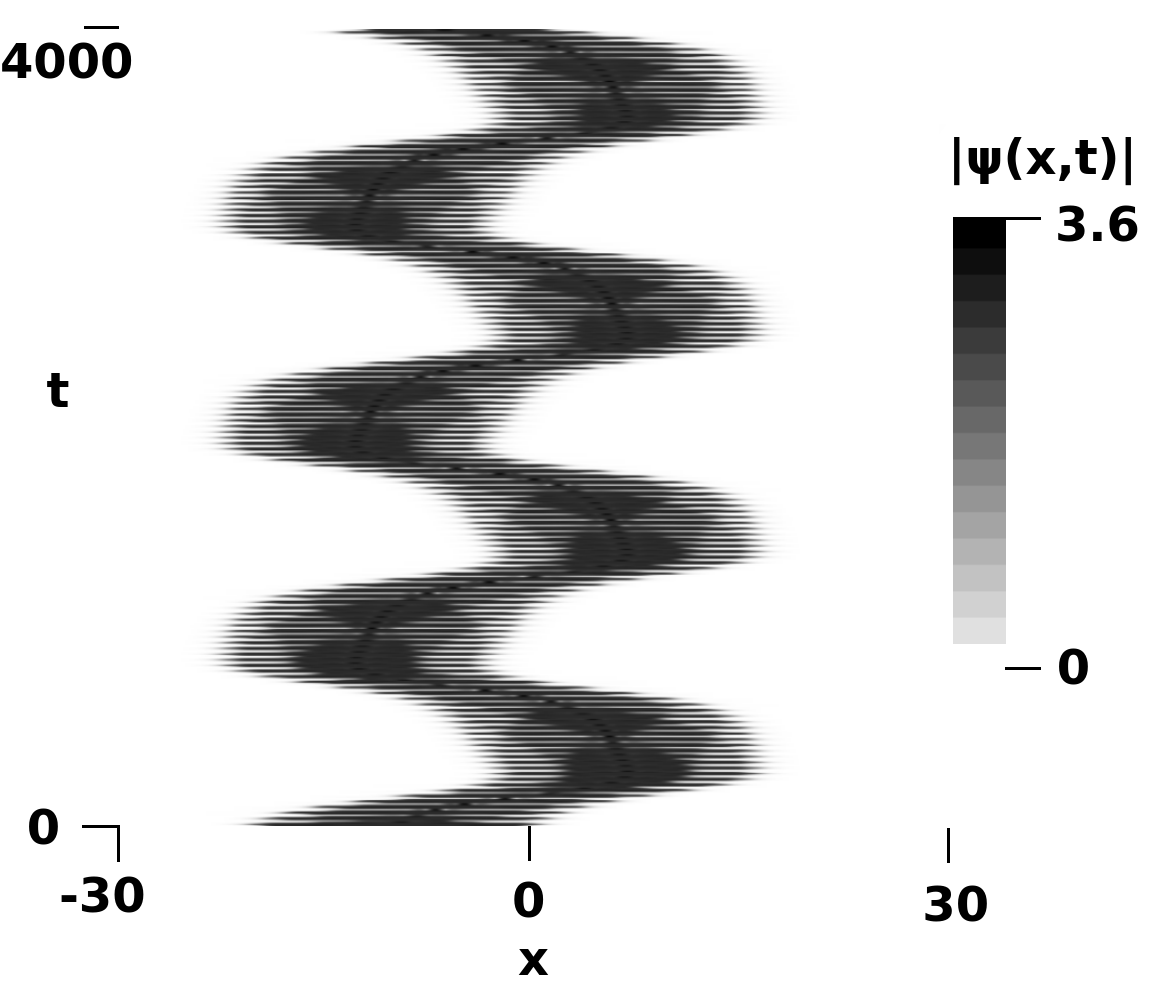
\includegraphics[width=3.6in]{periodpulse}
\caption{A creeping, pulsating soliton that is also periodic. Note that the unusual patterning inside the image is from aliasing. The parameters are $\epsilon=1.3,\ \delta=-0.1,\ D=1, \ \beta=0.101, \ \mu=-0.3,\ \nu=-0.101$.\cite{2001}}
\label{periodpulse} 
\end{figure}
%I feel like I should add something like you can get two types with the same parameter








\chapter{Results from Machine Learning}
\section{Collecting the Data}
A Gaussian pulse was used as the initial condition for all the solutions and was propagated for 700 units of time. Information such as the width and maximum height was taken from the last 100 time units so that the transient behaviour is less likely to still be present. A time step of 0.01 and spatial resolution of 0.01 were used, as this gave reliable results for many examples. This does exclude some of the high amp pulses, but otherwise it would have taken too long to calculate. In the simulations, these dissipate to nothing and so are not included in the machine learning data. For each solution, the average frequency, maximum standard deviation, maximum height, maximum energy were recorded as well as the maximum difference in standard deviation and energy. The parameters were chosen by generating random numbers over the following ranges. These ranges were chosen as they covered a many of the examples given in \cite{2001}. 
$$\delta: (-0.5,0.1)$$
$$\beta: (0,0.2)$$
$$D: (-1.5,1.5)$$
$$\epsilon: (0.5,1)$$
$$\mu: (-0.13,-0.07)$$
$$\nu: (-0.09,-0.05)$$
\\
It should be noted though that not all solutions of the CGLE will be localised solitons. There are a range of parameters where solutions called fronts exist. Fronts are characterised by having an increasing width, and given enough time it is able to be as wide as you want. \cite{2001}
Solutions that take up a large proportion of the periodic range should also be ignored as otherwise unusual effects can arise caused by this periodicity. 
\begin{figure}[h]
\centering
\includegraphics[width=6in]{unwanted}
\caption{Both of these results are unwanted solutions to the CGLE for machine learning. Left: A front with parameters $\epsilon=0.8,\ \delta=-0.1,\ D=1, \ \beta=0.08, \ \mu=-0.95,\ \nu=-0.08$. Right: An unwanted solution in part caused by the periodic boundary condition. Parameters are $\epsilon=0.5,\ \delta=-0.12,\ D=1, \ \beta=0.01, \ \mu=-0.1,\ \nu=-0.05$. }
\label{unwanted} 
\end{figure} 
These solutions can be filtered in the following way. First, the mean is found and is set to be the centre of the periodic boundary. If 65\% of the energy was not within a quarter of the way to the mean, it was deemed to most likely be either a front or another solution that could be ignored for the machine learning algorithm. Examples of this are given in figure \ref{unwanted}. 
\\
\\
Of the solutions that were not discarded, around 28500 examples were found which were not stationary solitons and 1300 were deemed to be examples of pulsating solitons. 
60\% of this data was used to train the machine learning algorithm. 20\% was used for the cross validation (CV) as a way to determine the ideal number of polynomial features, and 20\% was used to determine the the final accuracy of the algorithm. If there are a small number of features, the algorithm will not be able to fit either the cross validation set or the training set well. If there are too many features, it will over fit the training data, resulting in a low cost for the training data and a high cost for the cross validation data. This is shown in figure \ref{cv}.

\begin{figure}[h]
\centering
\includegraphics[width=3in]{cv}
\caption{When the number of parameters is small, the algorithm does not fit either the training or the cross validation set well. In contrast, too many features results in the training set fitting well and the cross validation set fitting well. The ideal number of parameters occurs at the minima.}
\label{cv} 
\end{figure} 




\section{Results}
The machine learning algorithm was run including third order polynomial features (84 parameters) up to 9th order (5005 parameters). to try and get data that resembles figure \ref{cv}. By doing this, the ideal polynomial order can be determined. This data is in the appendix. 
\\\\
The ideal parameter was then used to determine the accuracy of the prediction with the test data. The only data property tested that had a reliable prediction was for the height of a stationary soliton. This could predict an answer within 2\% of the true value for 92\% of the data. The next closest was the maximum height of an pulsating soliton, which within 2\% for 67\% of the data and this went up to 95\% when a 5\% margin was given. Below is a summary of these results.
\begin{center}
\begin{tabular}{|l|l|l|l|}
\hline
Property & Percentage with & Percentage with\\ %& Percentage with \\
 &  error below 2\% & error below 5\% \\%& error below 10\% \\
\hline
Nonpulsating Height&92&98\\
Nonpulsating Energy&9&14\\
Nonpulsating S.D.&0&2\\
Pulsating max. Height&67&95\\
Pulsating max. S.D.&0&25\\
Pulsating max. Energy&8&20\\
Pulsating Frequency&9&19\\
Pulsating max. Energy Diff&6&8\\
Pulsating max. S.D. Diff &0&1\\
\hline
\end{tabular}
\\Table: The proportion of correct guesses at a 2\% threshold.
\end{center}
The worst fitting solutions were isolated to try and understand why so many of these were very poor. Most of the worst examples had multiple solitons evolving in parallel and so this would significantly skew the results for energy and standard deviation.
\\\\
One potential way to get around this would be to start of with a single soliton, and as it evolves, vary the parameters until it reaches the desired parameters. Since this would be a gradual process, it would be less likely to split up into multiple solitons, compared to an arbitrary initial pulse. This could also have the advantage of allowing for the high amplitude solitons, as the frequency could be monitored and the propagation time and resolution could be adjusted accordingly. 
\\\\
Alternatively, the number of peaks in the x direction could be counted. However solitons often have multiple local maxima and so the threshold for a peak would need to be set high so that solitons are not unnecessarily discarded.
\\\\
Something else that could be tried is to classify exploding or high amplitude solitons with a neural network or SVM. This could be done by setting a threshold increase from the base soliton to determine whether it is an exploding/high amplitude soliton. 
\\\\
Yet something else that could be looked at is the rate of expansion of fronts, and this could be modelled in a similar way to machine learning, however the issue with this is that a new method to discard other unwanted solutions would need to be found. 
\\\\
Another significant way to improve the accuracy for pulsating solitons would be to get more data. The stationary solitons went up to a significantly higher number of parameters. This could only be done without overfitting occurring as there was a large sample size. If we expect pulsating properties to be at least as complicated, then a significantly larger sample size must be used. The larger sample size was not available when running these training algorithms, as the computer being used to run the simulation was frequently being used by other people. 
\\\\
A final improvement would be to go through the list of features and remove those that contribute only a small amount to the total prediction. Especially with high order polynomials, this would speed up the predictions made by the algorithm



\unnum{chapter}{Conclusion}
The complex Ginzburg Landau equation was solved using a split step Fourier and Runge Kutta method. This was done after various different methods had been explored and was chosen as it was found to be widely used and efficient.\cite{2001, taha, bch}. A range of previously published solitons were successfully replicated including high amplitude pulses and spiny solitons. The Stanford university online course on machine learning was successfully with various techniques being explored in depth. Polynomial regression was chosen to predict properties of solitons, however the only property that could be predicted was the height of stationary solitons which was able to predict an answer within 2\% of the true value for 92\% of the test solitons. The next best was predicting the maximum height for pulsating solitons, ad this was able to get 95\% within 5\% of the true value. Various reasons were explored as to why this may be the case, with the most likely culprit being that some of the solitons would split and propagate in parallel. Ways to overcome this were suggested and other future projects involving machine learning to predict soliton properties were discussed. 





\unnum{chapter}{Appendix}
\begin{center}
\begin{tabular}{|l|l|l|}
\hline
Polynomial Order & Training Cost & CV Cost\\
\hline
4&0.0011&0.00104\\
5&0.000860&0.000815\\
6&0.000674&0.000700\\
7&0.000662&0.000663\\
8&0.000662&0.000667\\
\hline
\end{tabular}
\\Table 1: Table of cost for the height of stationary solitons.
\end{center}
\begin{center}
\begin{tabular}{|l|l|l|}
\hline
Polynomial Order & Training Cost ($\times 10^7$) & CV Cost($\times 10^7$)\\
\hline
4&3.59&3.75\\
5&3.57&3.76\\
6&3.54&3.78\\
\hline
\end{tabular}
\\Table 2: Table of cost for the standard deviation of stationary solitons.
\end{center}
\begin{center}
\begin{tabular}{|l|l|l|}
\hline
Polynomial Order & Training Cost & CV Cost\\
\hline
4&6.41&7.03\\
5&5.73&6.49\\
6&5.40&6.21\\
7&5.05&6.03\\
8&4.74&5.55\\
9&4.72&5.72\\
\hline
\end{tabular}
\\Table 3: Table of cost for the energy of stationary solitons.
\end{center}
\begin{center}
\begin{tabular}{|l|l|l|}
\hline
Polynomial Order & Training Cost & CV Cost\\
\hline
3&41.2&56.1\\
4&33.9&131.9\\%TODO
5&28.8&85.3\\
\hline
\end{tabular}
\\Table 4: Table of cost for the maximum energy difference of pulsating solitons.
\end{center}
\begin{center}
\begin{tabular}{|l|l|l|}
\hline
Polynomial Order & Training Cost & CV Cost\\
\hline
3&5.3&2.3\\
4&4.6&6.1\\
5&4.1&6.5\\
\hline
\end{tabular}
\\Table 5: Table of cost for the maximum difference in standard deviation of pulsating solitons.
\end{center}
\begin{center}
\begin{tabular}{|l|l|l|}
\hline
Polynomial Order & Training Cost ($\times 10^7$) & CV Cost($\times 10^7$)\\
\hline
3&0.00178&0.00265\\
4&0.00152&0.00445\\
5&0.00133&0.00373\\
6&0.00118&0.00451\\
\hline
\end{tabular}
\\Table 6: Table of cost for the average frequency of pulsating solitons.
\end{center}
\begin{center}
\begin{tabular}{|l|l|l|}
\hline
Polynomial Order & Training Cost & CV Cost\\
\hline
3&0.00259&0.00495\\
4&0.00213&0.00896\\
5&0.00183&0.00714\\
6&0.00165&0.00743\\
\hline
\end{tabular}
\\Table 7: Table of cost for the maximum height of pulsating solitons.
\end{center}
\begin{center}
\begin{tabular}{|l|l|l|}
\hline
Polynomial Order & Training Cost  & CV Cost\\
\hline
3&30.9&52.5\\
4&25.2&84.3\\
5&20.2&75.8\\
6&17.2&64.9\\
7&14.8&66.7\\
\hline
\end{tabular}
\\Table 8: Table of cost for the maximum energy of pulsating solitons.
\end{center}
\pagebreak
\begin{center}
\begin{tabular}{|l|l|l|}
\hline
Polynomial Order & Training Cost ($\times 10^5$) & CV Cost($\times 10^5$)\\
\hline
3&510&663\\
4&454&838\\
5&417&816\\
\hline
\end{tabular}
\\Table 9: Table of cost for the maximum standard deviation of pulsating solitons.
\end{center}


\begin{thebibliography}{9}
\addcontentsline{toc}{chapter}{Bibliography} 
\bibitem{2001}
    N. Akhmediev, J. M. Soto-Crespo and G. Town, Phys. Rev. E 63, 056602 (2001)
\bibitem{taha}
	T. Taha and M. Ablowitz, Journal of Computational Physics, Volume 55, Issue 2 (1984)
\bibitem{dissys}
    K. Porsezian and V.C. Kuriakose, \emph{Optical Solitons: Theoretical and Experimental Challenges}, Springer 2002 (pp116)
\bibitem{spiny}
	Wonkeun Chang, Jose M. Soto-Crespo, Peter Vouzas, and Nail Akhmediev, "Spiny solitons and noise-like pulses," J. Opt. Soc. Am. B 32, 1377-1383 (2015)
\bibitem{spike}
	Wonkeun Chang, Jose M. Soto-Crespo, Peter Vouzas, and Nail Akhmediev, "Extreme amplitude spikes in a laser model described by the complex Ginzburg–Landau equation," Opt. Lett. 40, 2949-2952 (2015)
\bibitem{extreme}
	Wonkeun Chang, Jose M. Soto-Crespo, Peter Vouzas, and Nail Akhmediev
Phys. Rev. E 92, 022926 (2015)
\bibitem{5th}
	J. Moores, Optics Communications 96 (1993) pp65-70
\bibitem{wocgle}
	I. Aranson, L. Kramer, Reviews of Modern Physics,, Vol74 (2002) pp99
\bibitem{boyce}
	W. Boyce and R, DiPrima \emph{Elementary Differential Equations and Boundary Value Problems} 9th ed. John Wiley \& Sons Inc. (2009) pp459 
\bibitem{annett}
	J.Annett, \emph{Superconductivity, Superfluids and Condensates} Oxford University Press (2004) pp67
\bibitem{hecke}
	M. van Hecke and W. van Saarloos, \emph{Amplitude equations for pattern forming systems}, from \emph{Fundamental Problems in Statistical Mechanics VIII} (1994).
\bibitem{exact}
	Y. Peng and E Krishnan, Commum Math Sci Vol. 5 NO. 2 pp243-252 (2007)
\bibitem{bch}
	A. Torcini, H. Frauenkron and P. Grassberger, Physica D Vol. 103 (1997) pp605-610
\bibitem{mooc}
A. Ng, Stanford University, \url{https://www.coursera.org/learn/machine-learning}
	
\end{thebibliography}

\end{document}